\section*{Preface: Bridging Text between Chapters 3 and 4}
\addcontentsline{toc}{section}{Preface: Bridging Text between Chapters 3 and 4}


The method implemented in the previous chapter was used to study CNVs in low-mappability region.
The main challenge with low-mappability regions is the complex coverage profiles.
Because of the repeated sequences, the number of uniquely mapped reads is reduced and fluctuates depending on which repeats are present in each region.
Instead of attempting to model this complex sequence contexts, we use the population-based approach implemented in chapter \ref{chap:epi}, {\sf PopSV}, to robustly call CNVs in these challenging regions.
Indeed, the complex coverage profiles in low-mappability regions are consistent across samples from the same sequencing project.
Hence, if the read coverage in a sample is different enough from the reference samples, it is likely due to a CNV.

This manuscript was published in {\it Nucleic Acids Research}\cite{Monlong2018nar}.
First, we showed that {\sf PopSV} performance was preserved in low-mappability regions by consistently showing a high sensitivity and a stable false positive rate across different repeat profiles.
Using CNVs across 640 normal genomes we also showed that CNVs are enriched in low-mappability regions independently from the known enrichment in segmental duplication.
Thanks to the population-based approach, we provided a catalog of germline CNV that includes repeat-rich regions, including thousands of regions with recurrent variants that were missing from existing CNV databases.
\nameref{append:rep} contains supplementary tables, graphs and information.

\newpage
\singlespacing

\begin{center}
  \LARGE\bf Human copy number variants are enriched in regions of low mappability
\end{center}
\bigskip

\large{Jean Monlong$^{1,2}$, Patrick Cossette$^{3}$, Caroline Meloche$^3$, Guy Rouleau$^4$, Simon L. Girard$^{1,3,5}$, Guillaume Bourque$^{1,2,6}$}
\bigskip

\footnotesize
$^1$Department of Human Genetics, McGill University, Montr\'eal, H3A 1B1, Canada

$^2$Canadian Center for Computational Genomics, Montr\'eal, H3A 1A4, Canada

$^3$Centre de Recherche du Centre Hospitalier de l'Universit\'e de Montr\'eal, Montr\'eal, H2X 0A9, Quebec, Canada.

$^4$Montreal Neurological Institute, McGill University, Montr\'eal, H3A 2B4, Quebec, Canada.

$^5$D\'epartement des sciences fondamentales, Universit\'e du Qu\'ebec \`a  Chicoutimi, Chicoutimi, G7H 2B1, Canada

$^6$McGill University and G\'enome Qu\'ebec Innovation Center, Montr\'eal, H3A 1A4, Canada

\normalsize
\doublespacing

\section{Abstract}
Copy number variants (CNVs) are known to affect a large portion of the human genome and have been implicated in many diseases.
Although whole-genome sequencing (WGS) can help identify CNVs, most analytical methods suffer from limited sensitivity and specificity, especially in regions of low mappability.
To address this, we use {\sf PopSV}, a CNV caller that relies on multiple samples to control for technical variation.
We demonstrate that our calls are stable across different types of repeat-rich regions and validate the accuracy of our predictions using orthogonal approaches.
Applying {\sf PopSV} to 640 human genomes, we find that low-mappability regions are approximately 5 times more likely to harbor germline CNVs, in stark contrast to the nearly uniform distribution observed for somatic CNVs in 95 cancer genomes.
In addition to known enrichments in segmental duplication and near centromeres and telomeres, we also report that CNVs are enriched in specific types of satellite and in some of the most recent families of transposable elements.
Finally, using this comprehensive approach, we identify 3,455 regions with recurrent CNVs that were missing from existing catalogs.
In particular, we identify 347 genes with a novel exonic CNV in low-mappability regions, including 29 genes previously associated with disease.   


\section{Introduction}

%% Introduce SV/CNV and their importance
Genomic variation of 50 base pairs or more are collectively known as structural variants (SVs) and can take several forms including deletions, duplications, novel insertions, translocations and inversions\cite{Hall2012}.
Copy number variants (CNVs) are unbalanced SVs, i.e. affecting DNA copy number, and include deletions and any type of duplications (tandem duplications, triplications and other amplifications).
A wide range of mechanisms can produce SVs and is responsible for the diverse SV distribution across the genome, both in term of location and size\cite{Hall2012,Sharp2006,Mills2011}.
In healthy individuals, SVs are estimated to cumulatively affect a higher proportion of the genome as compared to single nucleotide polymorphisms (SNPs) \cite{Pang2010}.
SVs have been associated with numerous diseases including Crohn's Disease\cite{McCarroll2008a}, schizophrenia\cite{Stone2008}, obesity\cite{Bochukova2010}, epilepsy\cite{Mefford2011}, autism\cite{Stefansson2014}, cancer\cite{Beroukhim2010} and other inherited diseases \cite{Balzola2010,Ayarpadikannan2014}, and many SVs have a demonstrated detrimental effect. 

%% WGS and its challenges
While large SVs have been first studied using cytogenetic approaches and array-based technologies, whole-genome sequencing (WGS) is in theory capable of detecting SVs of any type and size\cite{Alkan2011}.
Numerous methods have been implemented to detect SVs from WGS data using either paired-end information\cite{Chen2009,Lindberg2014}, read-depth (RD) variation\cite{Boeva2011,Abyzov2011,Klambauer2012}, breakpoints detection through split-read approach\cite{Ye2009} or de novo assembly\cite{Rimmer2014}.
CNVs, potentially the most impactful SVs, can be detected by any of these strategies but are often resolved with a RD approach as it directly looks for signs of copy number changes.
However, several features of WGS experiments result in technical bias and continue to be a major challenge.
For example, GC content\cite{Benjamini2012}, mappability\cite{Treangen2011,Teo2012}, replication timing\cite{Koren2014}, DNA quality and library preparation\cite{VanDijk2014} have a detrimental impact on the uniformity of the RD\cite{Cheung2011}.
Unfortunately, this variability is difficult to fully correct for as it involves different factors, some of which are unknown, that vary from one experiment to another.
This issue particularly impairs the detection of CNV with weaker signal, which is inevitable in regions of low-mappability that represent around 10\% of the human genome\cite{Derrien2012}, for smaller CNVs or in cancer samples with cell heterogeneity or stromal contamination.
As a result, existing approaches suffer from limited sensitivity and specificity\cite{Mills2011,Alkan2011}, especially in regions of low-complexity and low-mappability\cite{Treangen2011,Teo2012}.
Even when problematic regions were masked and state-of-the-art bias correction\cite{Benjamini2012,Scheinin2014} were applied, we showed that technical variation in RD could still be found across three WGS datasets studied\cite{Monlong2018}.

%% Introduce PopSV's approach and compare with other methods
To control for technical variation, we recently developed a CNV detection method, {\sf PopSV}, which uses a set of reference samples to detect abnormal RD\cite{Monlong2018}. 
In each genome tested, the RD in a region is compared to the same region in the reference samples.
{\sf PopSV} differs from most previous RD methods, such as {\sf RDXplorer}\cite{Yoon2009} or {\sf CNVnator}\cite{Abyzov2011}, that scan the genome horizontally and look for regions that diverge from the expected global average.
Even when approaches rely on a ratio between an aberrant sample and a control, such as {\sf FREEC}\cite{Boeva2011} or {\sf BIC-seq}\cite{Xi2011}, we showed that they do not sufficiently control for experiment-specific noise as compared to {\sf PopSV}\cite{Monlong2018}.
Glusman et al.\cite{Glusman2015} does go further and normalize the RD with pre-computed RD profiles that fit the GC-fingerprint of a sample but this approach excludes regions with extreme RD and does not integrate the variance observed in individual regions. % which is essential to robustly deal with mappability bias.
{\sf PopSV} is also different from approaches such as {\sf cn.MOPS}\cite{Klambauer2012} and {\sf Genome STRiP}\cite{Handsaker2015} that scan simultaneously the genome of several samples and fit a Bayesian or Gaussian mixture model in each region.
Those methods have more power to detect CNVs present in several samples but may miss sample-specific events.
Moreover, their basic normalization of the RD and fully parametric models forces them to conceal a sizable portion of the genome and variants with weaker signal.
%% Ensemble approach
Finally, another strategy to improve the accuracy of CNV detection has been to use an ensemble approach that combines information from different methods relying on different types of reads.
Large re-sequencing projects such as the 1000 Genome Project\cite{Sudmant2015a,Mills2011} and the Genomes of Netherlands (GoNL) project \cite{Francioli2014,Kloosterman} have adopted this strategy and have successfully identified many CNVs using an extensive panel of detection methods combined with low-throughput validation.
Such a strategy increases the specificity of the calls at the cost of sensitivity.

Notably, with most of the tools and approaches described above, repeat-rich regions and other problematic regions of the genome are often removed or smoothed at some step of the analysis, to improve the accuracy of the calls. Although some methods\cite{Hormozdiari2010,He2011} try to model ambiguous mapping and repeat structure, only particular situations are addressed and, as a consequence, low-mappability regions are just scarcely covered in the most recent CNV catalogs\cite{Sudmant2015a}. This is unfortunate given that CNVs in such regions have already been associated with various diseases\cite{Ayarpadikannan2014,MacDonald1993,Rich2014,Mirkin2007,Carvalho2016} and that these regions are also more likely variable.
%% Expand on repeats
Indeed, different types of genomic repeats are likely to contribute to CNV formation.
For example, CNVs are known to be enriched in segmental duplications\cite{Sharp2006} and short and long tandem repeats are also known to be highly polymorphic\cite{Gymrek2012,Warburton2008}. Moreover, repeat templates, like segmental duplications or transposable elements, can facilitate the formation of CNV through non-allelic homologous recombination and other mechanisms\cite{Korbel2007}.

%% Outline - What's new since EpiPopSV ?
Given these facts and the growing realization of the importance of repetitive regions in the genome\cite{Hannan2018,Kazazian2017}, we wanted to investigate the performance of {\sf PopSV} in low-mappability regions and explore the comprehensive CNV distribution across a large cohort of healthy individuals.
After showing that population-based RD measures are better than existing mappability estimates to correct for variable coverage, we apply {\sf PopSV} to 640 WGS individuals from three human cohorts.
We compare the performance of {\sf PopSV} on these datasets with existing CNV detection methods in regions of low-mappability and validate the quality of the predictions across different repeat profiles using PCR validation.
Additionally, using publicly available long-read sequencing data and assemblies, we show that {\sf PopSV} is able to detect some highly ambiguous CNVs.
Next, having demonstrated the quality of the {\sf PopSV} calls, we characterize the patterns of CNVs across the human genome and produce a CNV catalog where variants of different types are better represented compared to existing catalogs.
We further find that CNVs are significantly enriched in regions of low-mappability and in different classes of repeats.
Finally, we identify novel CNV regions in low-mappability regions that were absent from previous CNV catalogs and describe their impact on protein-coding genes.

\section{Material and Methods}

\paragraph{Data}
Three publicly available WGS datasets were used.
The first is a twin study\cite{Boivin2013} with an average depth of 40x across 45 French-Canadian individuals, including 10 families of parents and monozygotic twins.
The second is a renal cell carcinoma dataset\cite{Scelo2014} (CageKid) with 95 tumor/normal pairs from four European countries and an average depth of 54x.
The third contains 500 unrelated Dutch individuals from the GoNL\cite{Francioli2014} dataset with an average depth of 14x.
In each study, the sequenced reads had been aligned using {\sf bwa}\cite{Li2010}.
See \nameref{sec:suppmat:reppopsv} for more details on access and read processing.

\paragraph{Read count across the genome}
The genome was fragmented in non-overlapping bins of fixed size.
As a RD measure we used the number of properly mapped reads, defined as read pairs with correct orientation and insert size, and a mapping quality of 30 (Phred score) or more.
In each sample, GC bias was corrected by fitting a LOESS model between the bin's RD and the bin's GC content.
We used a bin size of 5 Kbp for most of the analysis.
When specified, we used smaller bin sizes of 500 bp or 2 Kbp.

\paragraph{RD and mappability estimates}
To compare RD and mappability estimates in the Twin study, we first removed bins with extremely high RD if deviating from the median RD by more than 5 standard deviation.
The RD across the different samples were then combined and quantile normalized.
For each bin, we computed the average RD and standard deviation across the samples.
We downloaded the mappability track for hg19\cite{Derrien2012} and computed the average mappability in each bin.
We compared the RD in one randomly selected sample with the mappability estimates and with the inter-sample RD average.
To correct for the variation explained by the mappability estimates we fitted a generalized additive model using a cubic regression spline between the mappability estimates and RD in the sample (see \nameref{sec:suppmat:reppopsv}).
With these estimations and the global standard deviation we computed a Z-score for each bin.
A similar set of Z-scores was computed using the inter-sample average and standard deviation.
The normality of these two Z-score distributions were compared in term of excess kurtosis and skewness.
The Z-score distributions were also compared in different mappability intervals.
Finally, 45 samples of each cohort were combined and their RD quantile normalized. 
The inter-sample RD mean and standard deviation were then computed separately in each cohort and compared with the mappability estimates and RD in the selected sample.

\paragraph{{\sf PopSV} approach for CNV detection}
{\sf PopSV} was first described and applied in a CNV analysis of epilepsy patients\cite{Monlong2018}.
Briefly, a set of samples are chosen as reference and used to guide the normalization of each bin.
After normalization the average RD and standard deviation in each bin are saved and used to transform the RD in all samples into Z-scores.
CNVs are called in each sample when the RD is significantly higher or lower than in the reference samples.
The Z-scores can be segmented using the circular binary segmentation\cite{Seshan2017} or after statistical testing at the bin level.
As recommended, {\sf PopSV} was run separately on each dataset to avoid false positives due to potential variation in sequencing protocols.
More details are available in the original publication\cite{Monlong2018} and in the \nameref{sec:suppmat:reppopsv}.
With {\sf PopSV} there is no filtering, masking, smoothing or altering of repeat-rich regions: all the regions with properly mapped reads are analyzed.

\paragraph{Coverage track and low-mappability regions}
The average RD in the reference samples, a feature used during CNV calling, was used as a coverage track.
Bins with a RD lower than 4 standard deviation from the median were classified as {\it low-mappability} (or {\it low coverage}).
To highlight the most challenging region, we also defined {\it extremely low coverage} regions if the average RD was lower than 100 reads.
We overlapped these regions with protein-coding genes and segmental duplications (see \nameref{sec:suppmat:reppopsv}), and computed the distance to the nearest centromere, telomere or assembly gap.
We also counted the number of protein-coding genes overlapping at least one low-coverage region.

\paragraph{CNV detection using other methods}
{\sf FREEC}\cite{Boeva2011} and {\sf CNVnator}\cite{Abyzov2011} were run on each sample separately starting from the BAM files and using the same bin size as for {\sf PopSV} (5 Kbp).
{\sf cn.MOPS}\cite{Klambauer2012} was run on the same GC-corrected bin counts than for {\sf PopSV} and samples from the same dataset were jointly analyzed.
After retrieving split reads using {\sf YAHA}\cite{Faust2012}, {\sf LUMPY}\cite{Layer2012} was run and we kept all the deletions and duplications larger than 300 bp.
\verb!BND! variants with both ends more than 300 bp apart in the same chromosome were also included as they could be CNVs lacking support to characterize their type properly.
See \nameref{sec:suppmat:reppopsv} for more details.

\paragraph{Clustering samples using the CNV calls}
The similarity between two samples is defined by the amount of sequence called in both divided by the average amount of sequence called (see \nameref{sec:suppmat:reppopsv}).
This distance is used for hierarchical clustering of the samples in the Twin study using different linkage criteria ({\it average}, {\it complete} and {\it Ward}).
The clustering was performed using calls in regions with extremely low coverage ($\le$100 reads on average in the reference samples) only.
The Rand index estimated the concordance between the clustering and the known pedigree, grouping the samples per family (see \nameref{sec:suppmat:reppopsv}).

\paragraph{Replication in twins}
For each twin and each method, a CNV call was defined as {\it replicated} if also found in the other monozygotic twin but in less than 50\% of the population to remove systematic errors.
The frequency was computed by counting samples with any overlapping CNVs.
In order to avoid missing calls with borderline significance, we used slightly less confident calls for the second twin (see \nameref{sec:suppmat:reppopsv}).
For each method, we computed the number and proportion of {\it replicated} calls per sample.
We computed these metrics using all the calls, calls in low-mappability regions only, calls in segmental duplications, calls overlapping annotated repeats and calls overlapping annotated satellites, all using a minimum overlap of 90\% of the call's sequence.
Finally, we computed the replication estimates for calls located at 1 Mbp or less from a centromere, telomere or assembly gap.

\paragraph{Replication between paired normal and tumor samples}
The same approach was applied in the renal cancer dataset.
Here, {\it replicated} calls were found in a normal sample and its paired tumor but in less than 50\% of the normal samples.

\paragraph{Replication estimates and reliable regions}
Using CNV calls found in less than 50\% of the population, we defined as {\it reliable} a 10 Kbp region where more than 90\% of the overlapping calls were {\it replicated} calls.
We then compared the number and proportion of reliable regions for each method and in different types of region.
As before, we compared regions overlapping low-mappability regions, segmental duplications, annotated repeats, satellites, or located at less than 1Mbp from a centromere, telomere or assembly gap.

\paragraph{Experimental validation}
A subset of variants in the Twin study were experimentally validated.
First, we randomly selected one-copy and two-copy deletions, among small ($\sim700$ bp) and large ($\sim4$ Kbp) variants among the calls produced with 500 bp and 5 Kbp bins.
The calls were visually inspected to design PCR primers (see \nameref{sec:suppmat:reppopsv}).
We randomly selected 20 regions from those with available PCR primers.
Next, we randomly selected deletions overlapping low-mappability regions and called in 6 samples or fewer.
Because RD could not be used efficiently to fine-tune the breakpoints' location, we retrieved the reads (and their pairs) mapping to the region and assembled them (see \nameref{sec:suppmat:reppopsv}).
We randomly selected 17 regions from those with PCR primers.
In addition to gel electrophoresis, the amplified DNA of some regions was sequenced by Sanger sequencing.

\paragraph{Analysis of CEPH12878}
High coverage PCR-free Illumina WGS data for 30 samples, including CEPH12878, was downloaded from the 1000 Genomes Project (1000GP)\cite{Sudmant2015a} (see \nameref{sec:suppmat:reppopsv}).
{\sf PopSV} was run using 5 Kbp bins and all the samples as reference.
Using the same coverage track as before we selected all deletions in CEPH12878 overlapping low-mappability regions (at least 90\% of the call).
We first looked for support in CEPH12878 assemblies that used Illumina short-read sequencing, BioNano Genomics genome maps and either single molecule sequencing from the Pacific Biosciences (PacBio) platform\cite{Pendleton2015} or 10X Genomics linked-read sequencing\cite{Mostovoy2016}.
For each selected deletion from {\sf PopSV}, we aligned the flanking reference sequences to the assemblies using {\sf BLAST}\cite{Camacho2009} (see \nameref{sec:suppmat:reppopsv}).
When both flanks could be mapped to a contig, we visually inspected MUMmer plots\cite{Kurtz2004} which either supported the deletion, the reference genome sequence or were too noisy to assess.
We further annotated the selected calls if they overlapped with the deletions identified in Pendleton et al.\cite{Pendleton2015} over a minimum of 1 Kbp.
Finally, we downloaded the corrected PacBio reads and built a local assembly and consensus around each selected {\sf PopSV} deletion (see \nameref{sec:suppmat:reppopsv}).
We visually inspected MUMmer plots of the assembled and consensus sequences to confirm the presence of the deletion.

\paragraph{CNV catalog}
We called CNVs separately in each cohort with {\sf PopSV} using as reference samples the 45 samples in the Twin study, the normal samples in the cancer dataset and 200 samples in the GoNL dataset.
For the Twin study and the renal cancer dataset, {\sf PopSV} was run using 500 bp bins and 5 Kbp bins.
Because of the lower sequencing depth, {\sf PopSV} was run using 2 Kbp bins and 5 Kbp bins for the GoNL dataset.
For each sample, calls from the 2 different runs were merged when consistent (see \nameref{sec:suppmat:reppopsv}).
To compute the total number of calls, we collapsed calls with a reciprocal overlap higher than 50\%.
The amount of sequence affected in a genome is computed by merging all the variants in the cohort and counting the affected bases in the reference genome.

\paragraph{Comparison with public CNV catalogs}
We retrieved autosomal deletions, duplications and CNVs from four public CNV catalogs derived from large-scale WGS surveys: the 1000GP SV catalog\cite{Sudmant2015a}, {\sf Genome STRiP}'s catalog from 847 individuals\cite{Handsaker2015}, {\sf Genome STRiP} calls in 148 high-depth WGS genomes\cite{Chiang2017}, and the GoNL SV catalog\cite{Francioli2014} (see \nameref{sec:suppmat:reppopsv}).
To compare the amount of CNV with {\sf PopSV}, we removed deletions smaller than 300 bp as well as variants with high frequency ($>80\%$).
We compared CNV frequency between the 620 unrelated samples and a down-sampled set of 620 randomly selected individuals from the 1000GP CNV catalog.
The frequency was derived for all the nucleotide that overlaps at least one CNV as the proportion of individuals with a CNV in this locus.
The frequency distribution was computed separately for the different CNV types.

\paragraph{Comparison with CNV catalogs from long-read studies}
The SV catalog from Chaisson et al.\cite{Chaisson2014} was downloaded and overlapped with the CNV catalogs from 1000GP and {\sf PopSV} results on our 640 genomes.
Here, the 1000GP catalog contained deletions, duplications and CNVs of any size and frequency.
Using control regions and logistic regression we tested for an enrichment of variants in the SV catalog from Chaisson et al.\cite{Chaisson2014} (see \nameref{sec:suppmat:reppopsv}).
The analysis was performed separately on deletions, duplications, low-mappability regions and extremely low-mappability regions.
The same analysis was performed using the SV catalog from Pendleton et al.\cite{Pendleton2015}.

\paragraph{Novel CNV regions}
Using the 620 unrelated individuals across the three cohorts, we selected CNVs present in more than 1\% of the population (7 individuals or more) and not overlapping any CNV in the 1000GP catalog\cite{Sudmant2015a}.
We used deletions, duplications and CNVs of any size and frequency from the 1000GP.
Novel CNVs were collapsed into novel CNV regions, i.e. contiguous regions in which each base is overlapped by at least one novel CNV.
The novel CNV regions were annotated using the low-mappability and extremely low-mappability tracks.
We also compared CNVs from the three other public CNV catalogs to the novel CNV regions.

\paragraph{Distance to centromere, telomere and assembly gaps}
The centromeres, telomeres and assembly gaps (CTGs) were retrieved from the {\sf gap} track in UCSC\cite{Rosenbloom2015}.
In chromosomes with missing telomere annotation, we defined the telomere as the 10 Kbp region at the ends of chromosome.
The distance from each variant to the nearest CTG was computed and represented as a cumulative proportion.
Because this distribution changes with the size of the variants, we sampled random regions in the genome with similar sizes and computed the same distance distribution (see \nameref{sec:suppmat:reppopsv}).
Thanks to this null distribution we were able to see if variants were located closer/further to CTG than expected by chance.

\paragraph{Enrichment in genomic features}
We tested for CNV enrichment in different genomic features: genes, exons, low-mappability regions, segmental duplications, satellites, simple repeats and transposable elements.
The different satellite families, frequent simple repeat motives, transposable element families and sub-families were also tested.
For each sample, we computed a fold-enrichment as the fold change in proportion of regions overlapping a feature between CNV and control regions (see \nameref{sec:suppmat:reppopsv}).
The significance was assessed using logistic regression on the CNV and control regions.
To control for the enrichment in segmental duplications we used control regions with similar overlap profile (see \nameref{sec:suppmat:reppopsv}).
We also added a variable representing the overlap with segmental duplications as a co-factor in the logistic regression model.
When numerous tests were performed, e.g. satellite families, simple repeat motives, transposable element families or sub-families, the P-values were corrected for multiple testing using Benjamini-Hochberg procedure.
Finally, for each CNV and control region, we computed the proportion of the region overlapped by satellites, simple repeats and transposable elements.

\paragraph{Overlap with gene annotation}
Exons of protein-coding genes and promoter regions (10 Kbp upstream of the transcription start site) were extracted from the Gencode annotation v19.
We counted how many genes overlapped a CNV in the population when considering exons only, exons and promoter region, or gene body and promoter region.
In addition, we computed these numbers using only genes associated with a disease or phenotype in the OMIM Morbid Map (Online Mendelian Inheritance in Man; \url{http://omim.org/}).
These numbers were also computed for CNVs that overlapped more than 90\% of various classes of repeats.
For example, Satellite-CNVs are CNVs with more than 90\% of their region annotated as satellites.

\section{Results}

\subsection*{Modeling RD using population-based measures instead of mappability scores}
When counting uniquely mapped reads, the mappability of a region is a major predictor of the observed RD.
Theoretical mappability estimates\cite{Derrien2012} strongly correlated with the RD in a sample but many regions with intermediate mappability diverged from the predicted levels of RD (Fig. \ref{fig:mapcov}).
By computing the average RD across the 45 samples from the Twin study in each 5 Kbp bin we found that this divergence is consistent across samples and not simply due to a high RD variance (Fig. \ref{fig:mapmean}).
\begin{figure}[htp]
  \begin{subfigure}[b]{.48\textwidth}
    \includegraphics[width=\linewidth, page=4]{figures/wgs-map-coverage-cohorts.pdf}
    \caption{}
    \label{fig:mapmean}
  \end{subfigure}
  \begin{subfigure}[b]{.48\textwidth}
    \includegraphics[width=\linewidth, page=5]{figures/wgs-map-coverage-cohorts.pdf}
    \caption{}
    \label{fig:znorm}
  \end{subfigure}

  \begin{subfigure}[b]{.48\textwidth}
    \includegraphics[width=\linewidth, page=6]{figures/wgs-map-coverage-cohorts.pdf}
    \caption{}
    \label{fig:zmap}
  \end{subfigure}
  \begin{subfigure}[b]{.48\textwidth}
    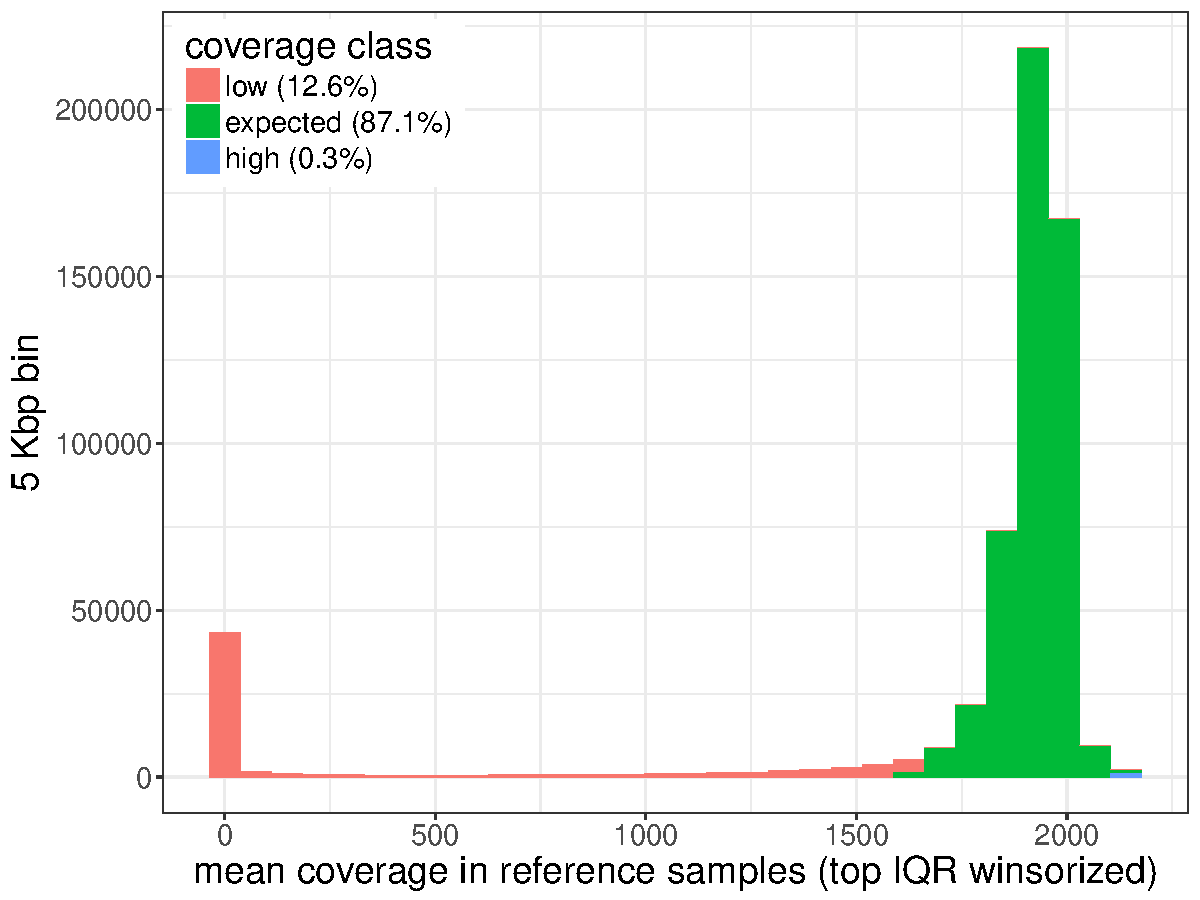
\includegraphics[width=\linewidth, page=1]{figures/wgs-coverage-tracks.pdf}
    \caption{}
    \label{fig:covclass}
  \end{subfigure}

  \caption[Mappability and population-based RD estimates.]{{\bf Mappability and population-based RD estimates.} {\small a) Inter-sample mean RD and average mappability in 5 Kbp bins. Regions with the same mappability estimate can have different RD levels. b) Z-score distribution. In {\it mappability}, Z-scores were computed from the mappability-predicted RD and global standard deviation; In {\it population estimates} from the inter-sample mean and standard deviation. c) Z-score distribution across the mappability spectrum. d) Average RD in the Twin study. The right-tail of the histogram was winsorized using the IQR and the different coverage classes are shown with colors.}}

\end{figure}
These mappability estimates only approximate RD variation and cannot explain the RD profile in numerous regions.
In contrast, population-based metrics more directly estimate the expected RD level (Fig. \ref{fig:meancov}).
Similarly to what was done in Monlong et al. in high-mappability regions\cite{Monlong2018}, we hypothesized that population-based estimates of RD mean and standard deviation could be used directly and help analyze regions with reduced RD.
To test this hypothesis, Z-scores corrected by the mappability-based estimates were compared to Z-scores derived from both the inter-sample mean and standard deviation.
The population-based Z-scores better followed a Normal distribution with an excess kurtosis of 0.2 and skewness of 0.004 compared to 29.4 and -2.284 respectively for mappability-adjusted Z-scores (Fig. \ref{fig:znorm}).
The distribution of the population-based Z-scores was also more stable across the mappability spectrum (Fig. \ref{fig:zmap}).
When comparing samples from the three different datasets, we noticed cohort-specific profiles in term of RD level and variance even though RD had been quantile normalized (Fig. \ref{fig:meancohort} and \ref{fig:sdcohort}), suggesting that population-based estimates will be better at capturing subtle cohort-specific variation.


These results suggest that a population-based strategy such as {\sf PopSV}\cite{Monlong2018} could be extended to investigate CNVs in regions of low-mappability.
To define low-mappability regions in the population, we used the average RD in the reference samples track produced by {\sf PopSV}.
In the Twin study for example, 12.6\% of the covered 5 Kbp bins were labeled as low-coverage (Fig. \ref{fig:covclass}), more than half of which were regions with extremely low coverage (lower than 100 reads on average).
Slightly fewer regions were labeled as low-coverage in the other cohorts (Fig. \ref{fig:covclass2}). As expected, low-coverage regions were depleted in gene content with only 15.3\% of the 5 Kbp bins in these regions overlapping a protein-coding gene versus 48.8\% for other regions. Nonetheless, 4,044 protein-coding genes overlapped a low-coverage region.
Finally, 23.2\% of the low-mappability regions overlapped segmental duplications and 69.1\% were located at less than 1 Mbp from a centromere, telomere or assembly gap, versus respectively 2.9\% and 8.8\% for other regions.

\subsection*{Replication rates in regions of low-mappability}
We previously demonstrated that CNV detection with {\sf PopSV} was overall more sensitive than {\sf FREEC}\cite{Boeva2011}, {\sf CNVnator}\cite{Abyzov2011}, {\sf cn.MOPS}\cite{Klambauer2012} and {\sf LUMPY}\cite{Layer2012} methods\cite{Monlong2018}.
In the following, we focused on the performance of {\sf PopSV} in low-mappability regions.
We first investigated the general concordance of the CNV calls with the pedigree in the Twin study.
Using calls in extremely low-mappability regions (average RD below 100 reads) only, we clustered the individuals and compared the result to the known pedigree.
We found that {\sf PopSV} showed better concordance, as assessed by the Rand index (Fig. \ref{fig:randindex}), compared to the other methods.
Indeed, the clustering dendogram from {\sf PopSV} calls, even in these challenging regions, captured almost perfectly the family relationships (Fig. \ref{fig:cluster}).
\begin{figure}[htp]
  \centering
  \begin{subfigure}[b]{\textwidth}
    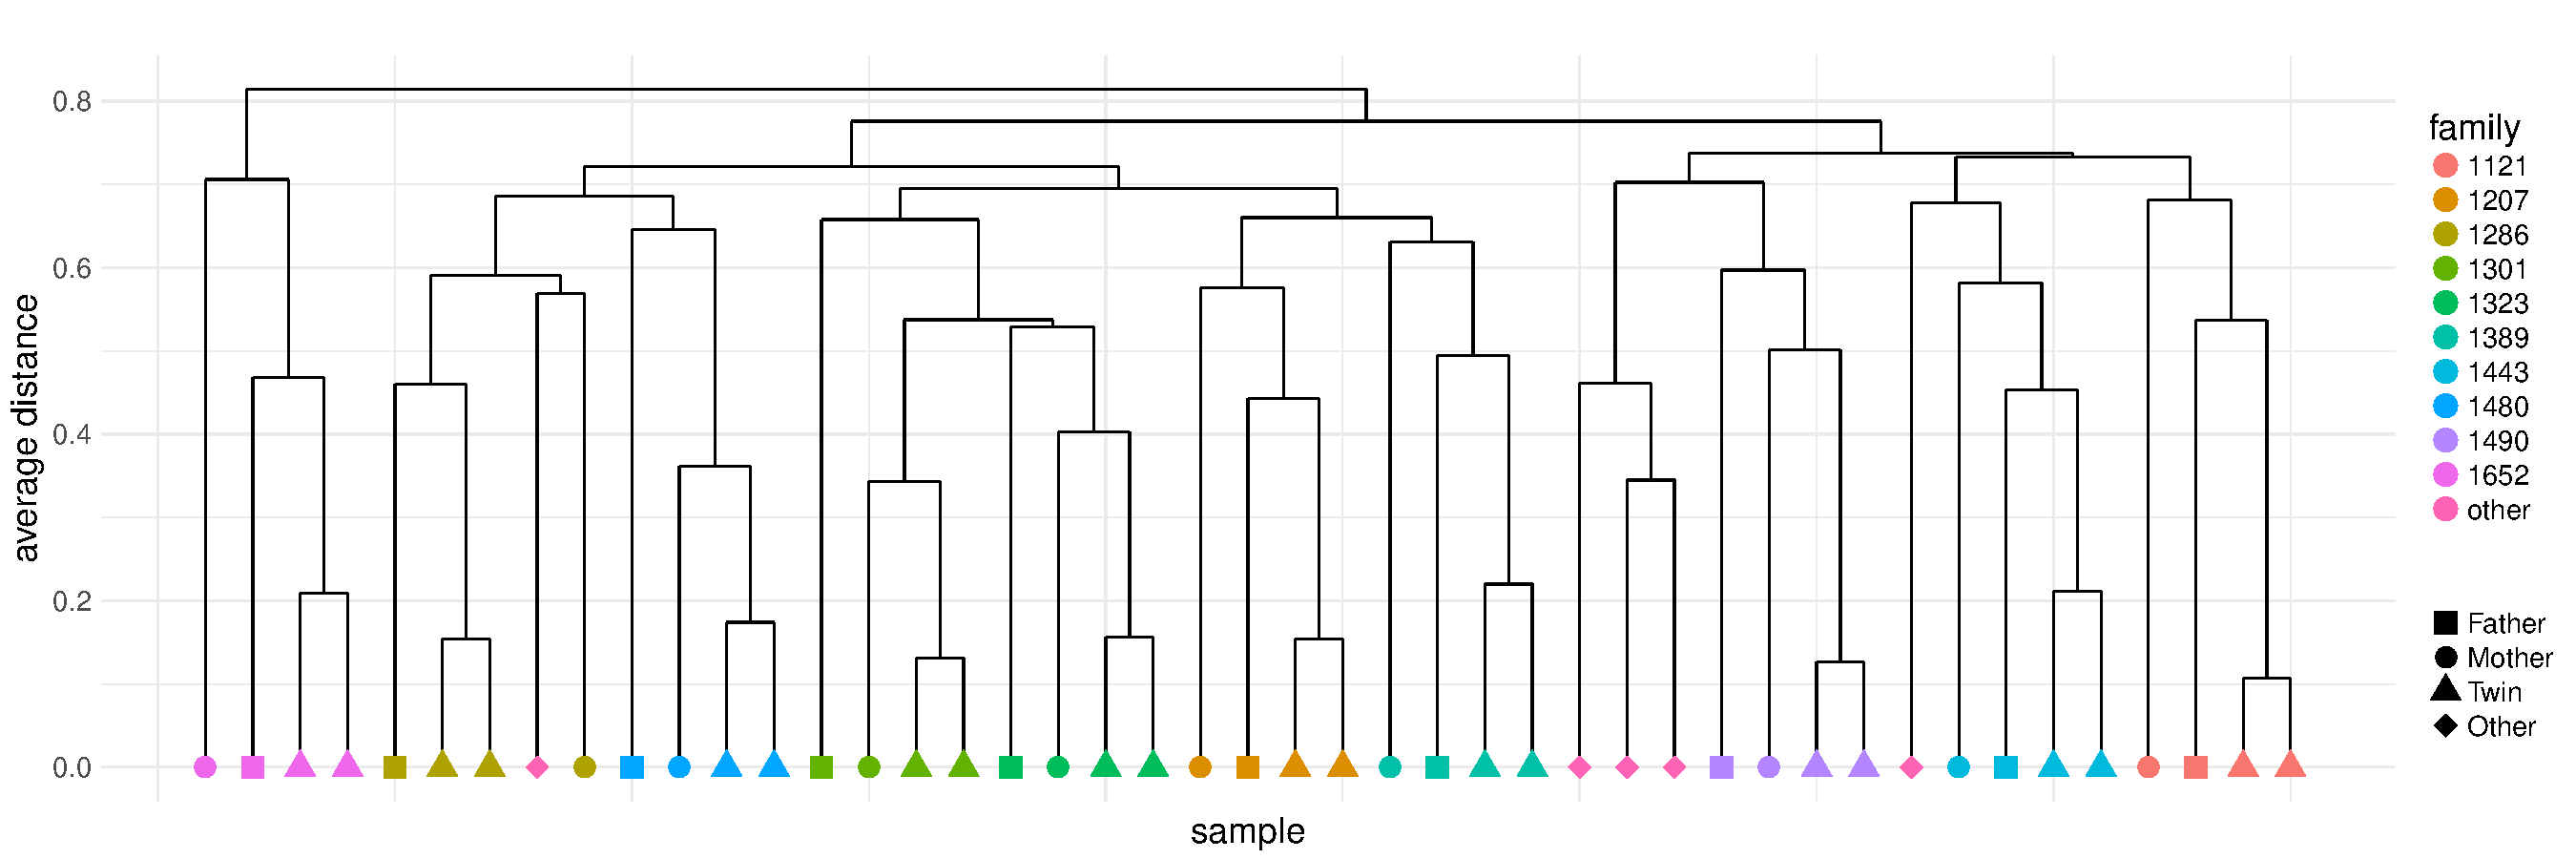
\includegraphics[width=\linewidth]{figures/replication-twins-long.pdf}
    \caption{}
    \label{fig:cluster}
  \end{subfigure}
  
  \begin{subfigure}[b]{.48\textwidth}
    \includegraphics[width=\linewidth, page=2]{figures/replication-twins.pdf}
    \caption{}
    \label{fig:replication}
  \end{subfigure}
  \begin{subfigure}[b]{.48\textwidth}
    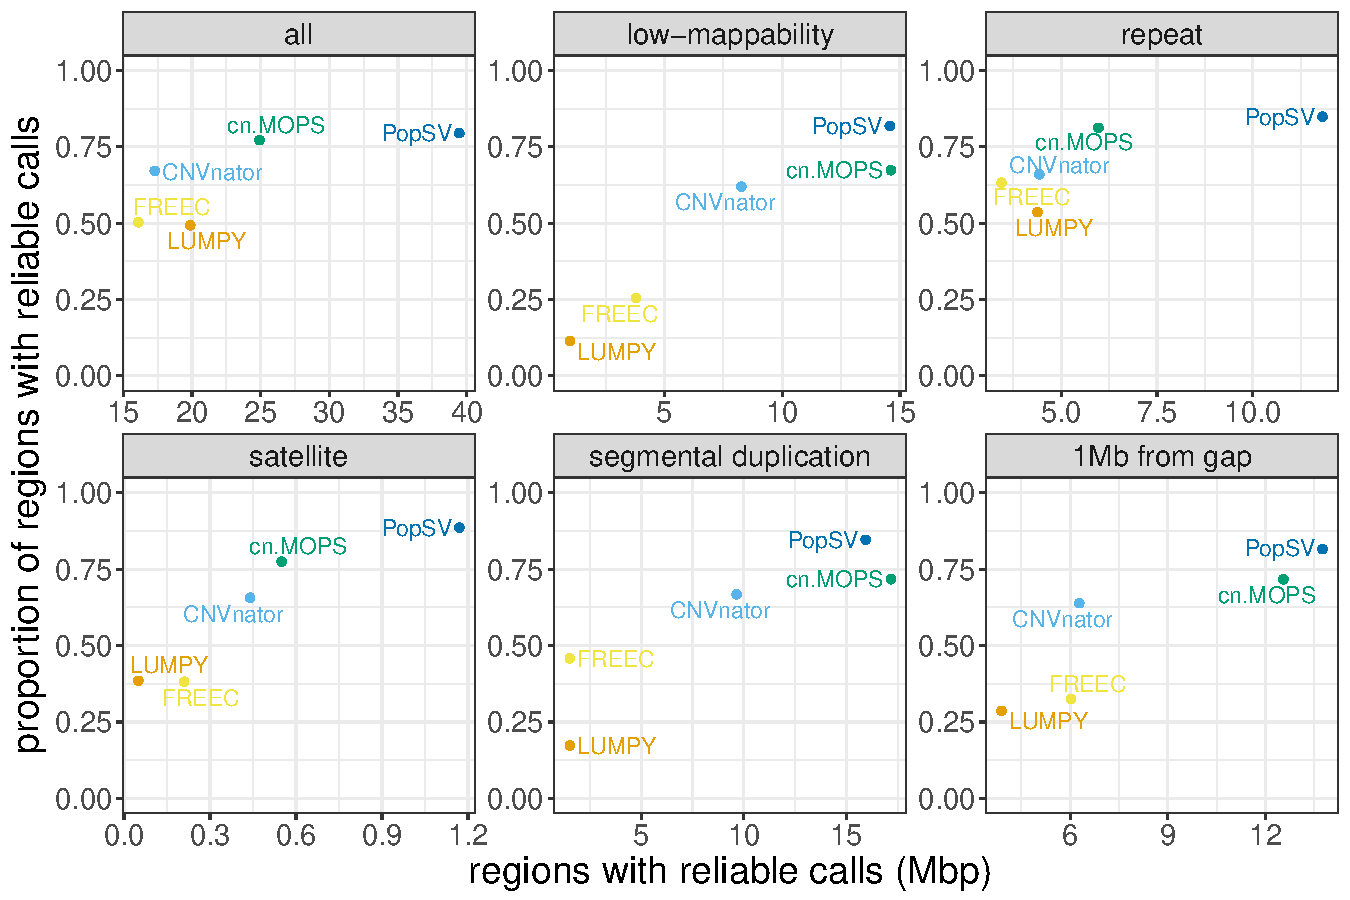
\includegraphics[width=\linewidth, page=1]{figures/replication-twins-reliable.pdf}
    \caption{}
    \label{fig:reliable}
  \end{subfigure}

  \caption[{\sf PopSV}'s performance in low-mappability regions.]{{\bf {\sf PopSV}'s performance in low-mappability regions.} {\small a) Cluster using {\sf PopSV} calls in extremely low coverage regions (below 100 reads). b) Proportion and number of calls replicated in the monozygotic twin. The point shows the median value per sample, the error bars the 95\% confidence interval. c) Proportion and number of regions with reliable calls, computed from call replication in twins.}}
\end{figure}
We then investigated if the call replication rate was stable across different mappability profiles.
Using calls present in less than 50\% of the population to avoid systematic bias, the overall replication rate in the other twin was found to be 89.7\%.
Focusing on calls in low-coverage regions, we found a comparable replication rate of 92.5\%.
The replication rate remained constant in regions with different repeat profiles (Fig. \ref{fig:replication}) such as regions overlapping segmental duplication, annotated repeats, or close to centromeres, telomeres and assembly gaps.
In contrast, the other methods showed a reduced replication and higher variance in repeat-rich regions.
The superior replication rate was complemented by a larger number of calls: {\sf PopSV} called between 2.7 and 9.9 times more replicated CNVs per sample in low-coverage regions compared to the other methods.
We observed the same results in the cancer dataset when comparing the agreement between germline events in normal/tumor pairs.
{\sf PopSV} had between 1.8 and 17.8 times more calls in low-mappability regions compared to the other methods and a stable replication rate across repeat profiles (Fig. \ref{fig:replication:cagekid}).
We next wanted to assess the performance in each region of the genome, rather than overall rates per sample, and used the replication in twins to identify regions with reliable calls.
Again we observed that {\sf PopSV} was as reliable overall as in regions with different repeat profiles (Fig. \ref{fig:reliable}).
This analysis also showed that {\sf PopSV} provides reliable calls in a larger fraction of the genome compared to other methods.
The strongest gain was observed for regions overlapping satellites or overlapping almost completely annotated repeats, with around twice as many regions reliably called by {\sf PopSV}.
{\sf cn.MOPS} showed the second best performance, especially in regions overlapping segmental duplications or close to centromeres, telomeres and assembly gap.

\subsection*{Validation of CNVs in regions of low-mappability}

% \paragraph{Experimental validation}
Using Real-Time PCR validation across 151 regions, we previously demonstrated that the replication estimates from the Twin dataset are consistent with experimental validation\cite{Monlong2018}.
We had tested variants of different types, sizes and frequencies and validated 90.7\% of the calls, similar to our twin-based replication estimates.
Here we tested additional deletions in individuals from the Twin study using PCR validation.
We first validated randomly selected deletions and found a validation rate close to the overall replication rate, with 18 out of 20 deletions (90\%) successfully validated (Table \ref{tab:pcr}).
In a second validation batch, we focused on rare deletions in low-mappability regions, of which 11 out of the 17 (65\%) were successfully validated (Table \ref{tab:pcr2}).
We noticed that the majority of the non-validated deletions were predicted to be smaller than 100 bp and most likely due to a problem during the breakpoint fine-tuning.
If we consider only deletions larger than 100 bp, the validation rate in regions of low-mappability increased to 83\% (10/12) once again close to {\sf PopSV}'s replication rates in the Twin dataset.

Regions with extreme repeat content remained difficult to target and validate using PCR approaches.
To further interrogate the performance of {\sf PopSV} in those regions, we turned to whole-genome data from long-read sequencing technology.
Publicly available assemblies for CEPH12878 samples confirmed several deletions called by {\sf PopSV} in low-mappability regions.
Out of the 14 homozygous deletions that could be assessed, 13 were confirmed in a contig, 12 of which were observed in both assemblies\cite{Pendleton2015,Mostovoy2016}.
Only one region seemed to be a false positive, an assembled contig supporting the reference sequence in one assembly.
Eleven regions could not be assessed because the flanks in the reference genome didn't map to any assembled contigs or their MUMmer plots neither supported a deletion nor the reference sequence.
In summary, we confirmed 92.8\% of the homozygous deletions in low-mappability regions that could be compared with the assemblies.
Deletions can be confirmed by direct comparison of the variant region and, if homozygous, should be present in the assembly.
In contrast, heterozygous deletions could be missing from an assembly if only the reference allele was assembled.
We confirmed 27 out of the 44 heterozygous deletions in low-mappability regions that could be assessed (Table \ref{tab:cephAss}).
As expected, only one allele was supported for many regions: 16 regions with only the deleted allele observed and 17 regions with only the reference allele observed.
Both deleted and reference alleles were observed for 11 variants.
Although only 61.3\% of the heterozygous deletion were confirmed, many variants might have been missed because of assembly preference to one allele, as suggested by the similar number of regions with only one supported allele.
Using variants identified by Pendleton et al.\cite{Pendleton2015} and by assembling raw PacBio reads, we found support for 3 additional homozygous deletions and 15 heterozygous deletions that had remained inconclusive in the assembly comparison.
Most of the regions that couldn't be confirmed were located close to assembly gaps in the reference genome (Fig. \ref{fig:cephGap}).
This observation highlighted that even with long-read sequencing data, it is not straightforward to clearly assess some genomic regions close to assembly gaps.

\subsection*{Global patterns of CNVs across the human genome}

Having demonstrated the robustness of {\sf PopSV} in low-mappability regions, we wanted to characterize the global patterns of CNVs across the human genome.
We were especially interested in looking at calls in regions of low-mappability which represents between 9-12\% of the human genome (Fig. \ref{fig:covclass} and \ref{fig:covclass2}).
We started with an analysis of the twins and the normal samples in the renal cancer dataset, both of which have an average sequencing depth around 40X.
{\sf PopSV} was used to call CNV using 500 bp and 5 Kbp bins, which were then merged to create a final set of variants.
On average per genome, 7.4 Mbp of the reference genome had abnormal read coverage, 4 Mbp showing an excess of reads indicating duplications and 3.4 Mbp showing a lack of reads indicating deletions (Table \ref{tab:res}).
\begin{sidewaystable}
  \resizebox{\textwidth}{!}{
    \begin{tabular}{|l|r|r|rrr|r|rr|rrrr|}
      \hline
      \multirow{2}{*}{Set}  & \multirow{2}{*}{Depth} & \multirow{2}{*}{Samples} & \multicolumn{3}{c|}{Variants} & \multirow{2}{*}{Avg Size (Kbp)} & \multicolumn{2}{c|}{Variants $<$3 Kbp} & \multicolumn{4}{c|}{Affected genome (Mbp)}                                       \\
                            &                        &                          & Total                         & \multicolumn{2}{c|}{Per sample} &                                        & Proportion & Per sample & Total   & \multicolumn{3}{c|}{Per sample}             \\
      \hline
                            &                        &                          &                               & {\it WG}                        & {\it ELC}                               &            &            &         &        & {\it min} & {\it mean} & {\it max} \\
                            % \hline


      Twin study            & 42x & 45  & 20,222 & 1,637.27 & 243.24 & 4.21 & 0.65 & 1,056.84 & 62.22  & 5.30 & 6.89 & 9.03  \\
      {\it ~~deletion}      &     &     & 10,661 & 727.04  & 13.20  & 4.53 & 0.58 & 423.80  & 33.97  & 2.79 & 3.30 & 3.85  \\
      {\it ~~duplication}   &     &     & 10,396 & 910.22  & 230.04 & 3.94 & 0.70 & 633.04  & 34.20  & 2.50 & 3.59 & 5.29  \\
      \hline                                                                                                                                                                  
      CageKid normals & 40x & 95  & 56,256 & 2,132.81 & 336.46 & 3.58 & 0.71 & 1,521.16 & 134.77 & 5.53 & 7.63 & 10.24 \\
      {\it ~~deletion}      &     &     & 25,367 & 805.08  & 12.74  & 4.30 & 0.63 & 508.56  & 70.65  & 2.65 & 3.46 & 7.26  \\
      {\it ~~duplication}   &     &     & 32,356 & 1,327.73 & 323.73 & 3.14 & 0.76 & 1,012.60 & 76.28  & 2.31 & 4.17 & 6.70  \\
      \hline                                                                                                                                                                  
      GoNL                  & 13x & 500 & 27,945 & 549.52  & 81.97  & 8.71 & 0.46 & 250.24  & 226.50 & 3.05 & 4.79 & 8.16  \\
      {\it ~~deletion}      &     &     & 13,818 & 262.41  & 1.45   & 8.50 & 0.42 & 110.16  & 106.83 & 1.30 & 2.23 & 3.96  \\
      {\it ~~duplication}   &     &     & 15,291 & 287.10  & 80.52  & 8.91 & 0.49 & 140.08  & 139.21 & 1.45 & 2.56 & 5.72  \\
      \hline
    \end{tabular}
  }
  \caption[CNVs in the Twins, CageKid normals and GoNL datasets.]{{\bf CNVs in the Twins, CageKid normals and GoNL datasets. }{\small WG: whole genome; ELC: extremely low-coverage regions. The {\it Total} number of variants is the total number after collapsing recurrent variants. {\it Affected genome} represents the amount of the reference genome that overlaps at least one CNV.}}
  \label{tab:res}
\end{sidewaystable}
In both datasets, the average variant size was around 3.7 Kbp and 70\% of the variants found were smaller than 3 Kbp.
We compared our numbers to equivalent CNVs detected in the most recent human SV catalog from the 1000 Genomes Project (1000GP), where 6.1 Mbp was found to be copy-number variable on average in each genome (Table \ref{tab:1kgp}).
In those calls, we notice that no variants except for a few deletions were identified in regions of extremely low-mappability regions.
Similarly, small duplications ($<3$ Kbp) were absent from that catalog.
In contrast, the set of variants identified by {\sf PopSV} included variants in extremely low-mappability regions as well as small deletions and duplications (Table \ref{tab:res}), explaining in part the $\sim20\%$ increase in affected genome.
While the study from the 1000GP\cite{Sudmant2015a} explored a wider range of SVs, our catalog is likely more representative of the distribution of CNVs in a normal genome since a larger portion of the genome could be analyzed.
Small duplications and events in low-mappability regions were also under-represented in more recent CNV surveys that used higher sequencing depth or joint-calling of CNVs\cite{Handsaker2015,Chiang2017,Francioli2014} (Table \ref{tab:1kgp}), confirming the uniqueness of the PopSV catalog.

Next, we applied {\sf PopSV} to the 500 unrelated samples from the GoNL cohort (Table \ref{tab:res}).
Due to a lower sequencing depth ($\sim$13X), we used bins of size 2 Kbp and 5Kbp, explaining the lower number of variants found in these samples.
Nevertheless, a large sample size helps better characterize the frequency patterns and provides a more comprehensive map of rare CNVs.
In total, across these three cohorts, 325.6 Mbp were found to be affected by a CNV with more duplications (50,856) detected than deletions (44,110).
This contrasts with the CNVs reported by the 1000GP\cite{Sudmant2015a} that were heavily skewed towards deletions (Table \ref{tab:1kgp}), likely due to the conservative ensemble approached used to detect CNVs.
The frequency distribution of deletions and duplications found using {\sf PopSV} were also much more balanced compared with the ones from the 1000GP\cite{Sudmant2015a} (Fig. \ref{fig:freq1kgp}).
\begin{figure}[htp]
  \centering
  \begin{subfigure}{.49\textwidth}
    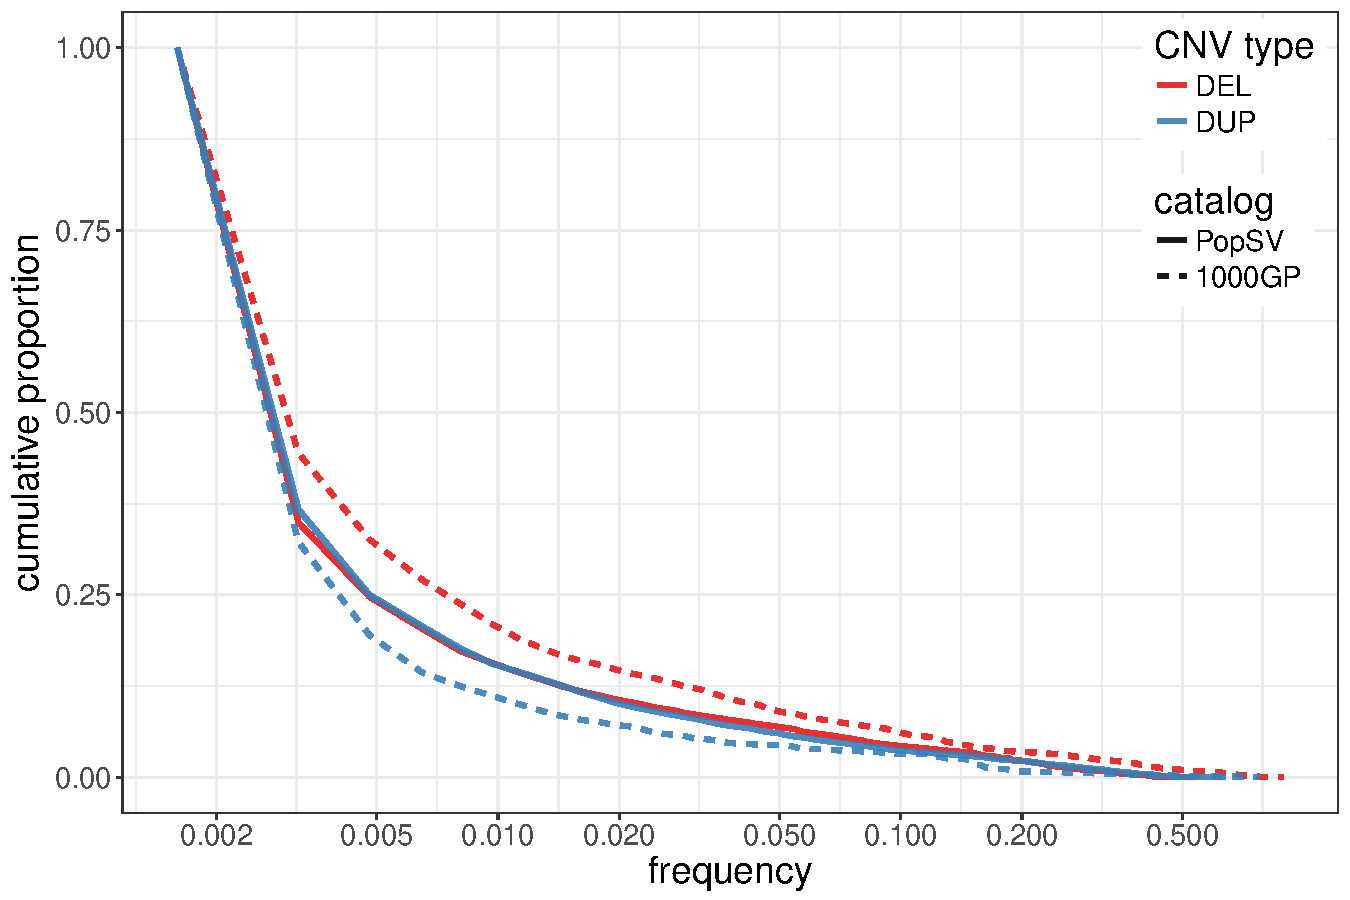
\includegraphics[width=\linewidth,page=1]{figures/PopSV-catalog-overview.pdf}
    \caption{}
    \label{fig:freq1kgp}
  \end{subfigure}
  \begin{subfigure}{.49\textwidth}
    \includegraphics[width=\linewidth,page=2]{figures/PopSV-catalog-overview.pdf}
    \caption{}
    \label{fig:chaisson}
  \end{subfigure}
  \caption[Comparison with CNV catalogs from the 1000 Genomes Project and a long-read sequencing study]{{\bf Comparison with CNV catalogs from the 1000 Genomes Project\cite{Sudmant2015a} (1000GP) and a long-read sequencing study\cite{Chaisson2014}.} {\small a) The x-axis represents the proportion of individuals with a CNV overlapping a region. The y-axis represents the cumulative proportion of the affected genome. b) Overlap with the SV catalog from Chaisson et al.\cite{Chaisson2014}. In each cohort (color), the proportion of collapsed calls overlapping calls from Chaisson et al.\cite{Chaisson2014} or control regions with similar size distribution was modeled using a logistic regression. Boxplots show variation across 50 sampling of control regions. {\it low-map}: calls in low-mappability regions; {\it ext. low-map}: calls in extremely low-mappability regions.}}
\end{figure}
We also compared our CNV catalog with an orthogonal set of calls from Chaisson et al.\cite{Chaisson2014} that were obtained using long-read sequencing.
Although these calls came from a different genome, we expect both catalogs to share a number of common variants.
We found a significant overlap between the two catalogs, overall and separately for deletions, duplications, low-mappability regions and extremely low-mappability regions (Fig \ref{fig:chaisson}).
In all categories, the overlap was stronger for {\sf PopSV}'s catalog compared to the 1000GP CNV catalog.
We noted that the enrichment for the 1000GP catalog disappeared for duplications and low-mappability regions but was even stronger for {\sf PopSV}'s catalog.
Like {\sf PopSV}, the long-read sequencing study\cite{Chaisson2014} also found a better balance between deletions and duplications.
Similar observations were made using another set of calls from long-read sequencing of the CEPH12878 sample\cite{Pendleton2015} (Fig. \ref{fig:pendcat}).

\subsection*{CNVs are enriched near centromeres and telomeres and in regions of low-mappability}

Large CNVs have been shown to be enriched near centromeres, telomeres and assembly gaps (CTGs)\cite{Nguyen2006}.
We were interested in exploring this observation further using the set of high resolution calls from {\sf PopSV}.
We compared the distribution of CNVs calls made across the 3 datasets to randomly distributed regions of similar sizes (Fig. \ref{fig:ctgDist}).
In an average genome, we found that 33.5\% of the CNVs calls were within 1 Mbp of a CTG, while we would have expected only 11.2\% by chance.
To verify that these observations were not simply a consequence of the methodology used, we also looked at the somatic CNVs (sCNVs) that we could detect in the renal cell carcinoma dataset.
For this purpose, we extracted the variants found by {\sf PopSV} in the tumor sample of an individual but missing from its paired normal sample.
Reassuringly, and in contrast to germline CNVs, sCNVs were not preferentially found near CTGs (Fig. \ref{fig:ctgDist}), with 11.1\% of the sCNVs within 1 Mbp of a CTG.

After correcting for the distance to CTGs, we also observed a 4.7 fold-enrichment of variants in regions of low mappability (Fig. \ref{fig:repAll}).
\begin{figure}[htp]
  \centering
  \begin{subfigure}{.9\textwidth}
  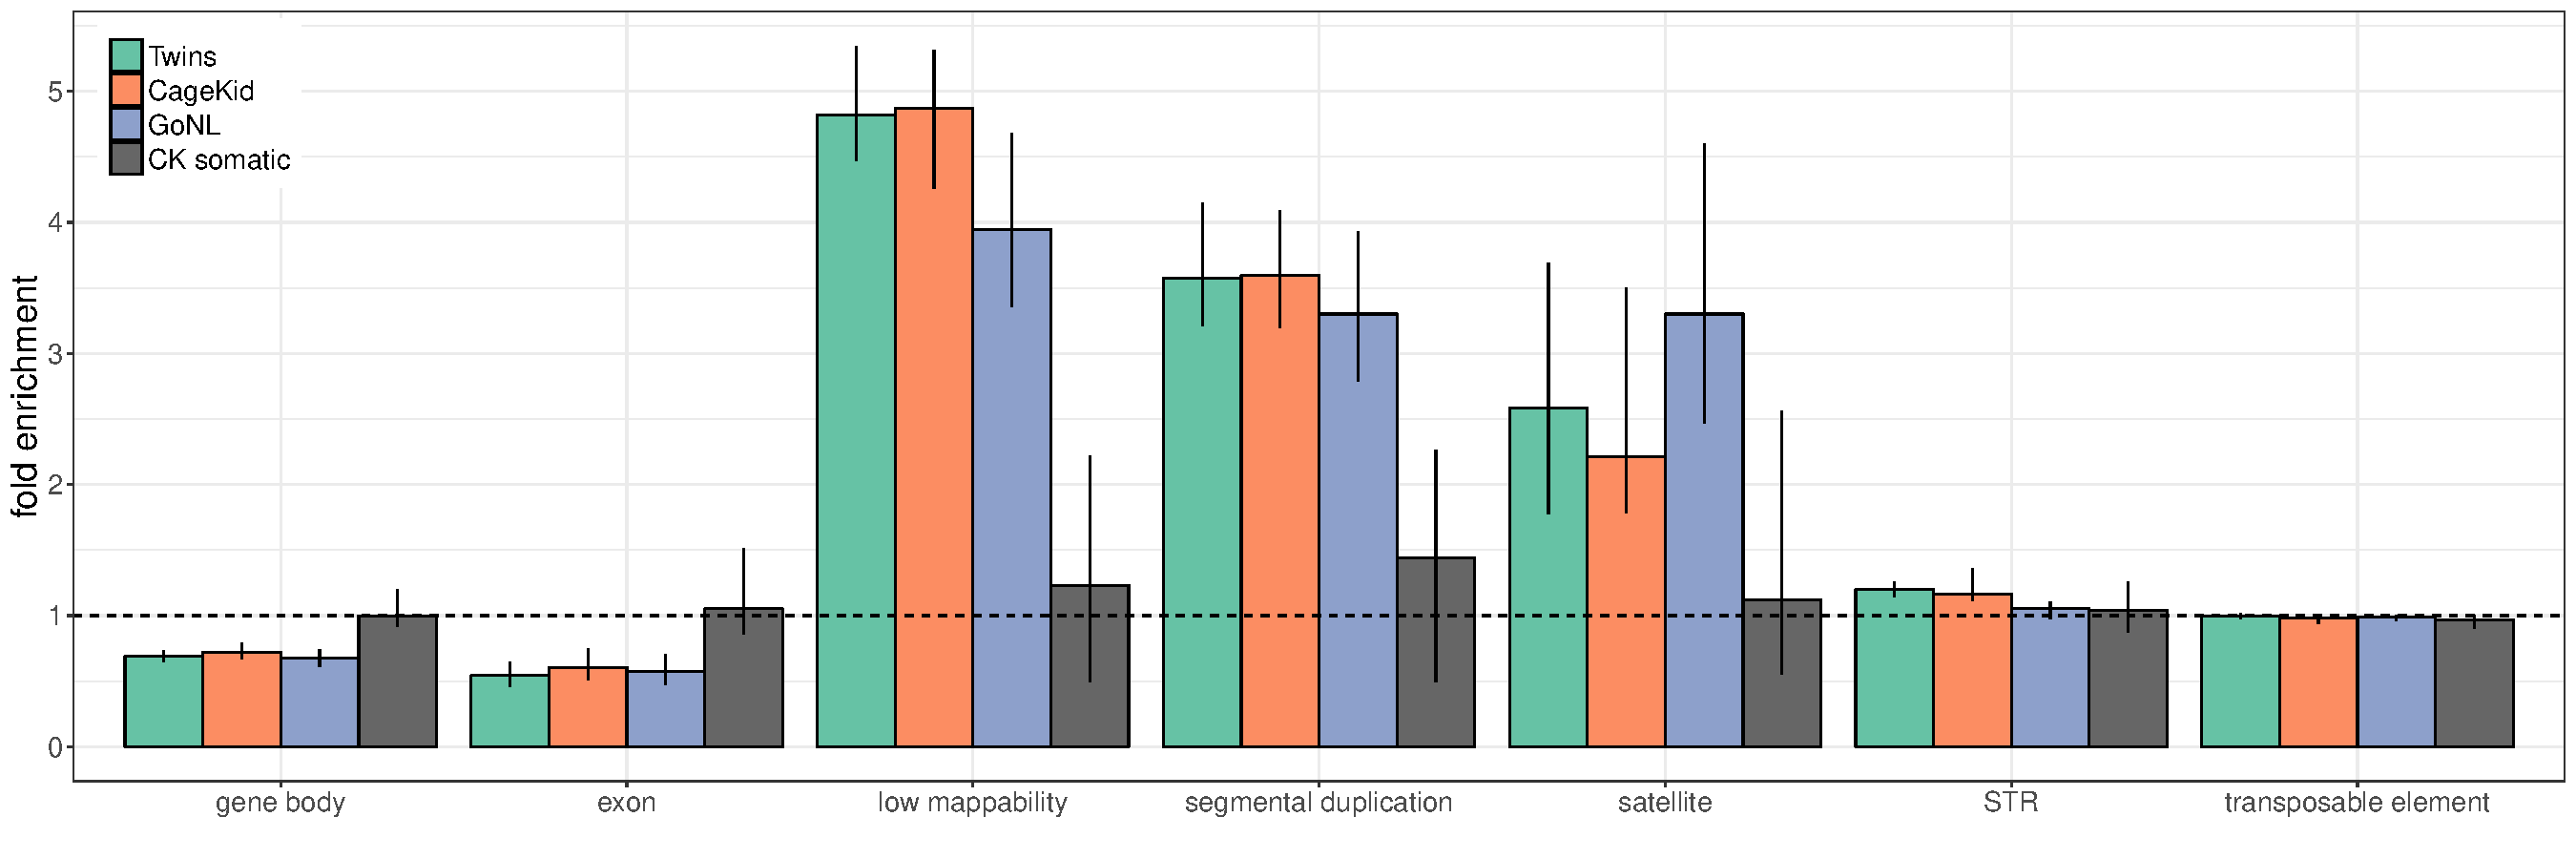
\includegraphics[width=\textwidth, page=1]{figures/PopSV-repeatEnr-long.pdf}
  \caption{}
  \label{fig:repAll}
  \end{subfigure}
  \begin{subfigure}{.9\textwidth}
  \includegraphics[width=\textwidth, page=3]{figures/PopSV-repeatEnr-long.pdf}
  \caption{}
  \label{fig:repFam}
  \end{subfigure}
  \caption[CNVs in normal genomes.]{{\bf CNVs in normal genomes.} {\small a) Enrichment of CNVs in different genomic classes (x-axis) across different cohorts (colors) and controlling for the distance to centromere/telomere/gap. Bars show the median fold enrichment compared to control regions. The error bar represents 90\% of the samples in the cohort. b) Enrichment of CNVs in repeat families (x-axis) controlling for the overlap with segmental duplication and distance to centromere/telomere/gap. The error bars were winsorized at 7 for clarity. {\it STR: Short Tandem Repeat}; {\it TE: Transposable Element}.
    }}
\end{figure}
Segmental duplications (SD), DNA satellites and Short Tandem Repeats (STRs) were also significantly enriched with fold-enrichment of 3.6, 2.6 and 1.2, respectively.
The over-representation of CNVs in SDs has been described before\cite{Sharp2006} and in a recent study \cite{Sudmant2015}, half of the CNV base pairs were shown to overlap a SD.
To investigate the contribution of low-mappability regions beyond SDs, we used matched control regions and included segmental duplication overlap in the logistic regression model.
Even after controlling for this known enrichment, we found that CNVs overlapped low-coverage regions more than twice as much as expected (Fig. \ref{fig:repCont}).
This two-fold enrichment is independent of the SD association and consistently observed in the 3 cohorts of normal genomes.
In contrast to germline CNVs, sCNVs were once again found to be more uniformly distributed (Fig. \ref{fig:repAll} and \ref{fig:repCont}).
These results suggest that the enrichments of germline CNVs near CTGs and in regions of low-mappability are unlikely to be the result of a methodological artifact.

\subsection*{Various repeat families are more prone to harbor CNVs}

We wanted to further characterize the distribution of germline CNVs in relation to different repeat classes and families.
By comparing CNVs to the same control regions with matched overlap with SD and distance to CTGs we can look for patterns that are specific to repeat sub-families without the risk of being biased by the global enrichments (Fig. \ref{fig:repFam}).
Using this approach, we found that CNVs were still significantly enriched in satellites repeats and in short tandem repeats (P-value $<10^{-4}$, Fig. \ref{fig:repCont}), with fold-enrichments of 2.3 and 1.2 respectively.

Although it is known that DNA satellites and simple repeats are more unstable\cite{Eckert2009}, the extent to which CNVs are found in these regions in humans had, to our knowledge, not been systematically explored.
Satellite repeats are grouped into distinct families depending on their repeated unit and we found that not all satellite repeats were equally likely to overlap a CNV (Fig. \ref{fig:repSat}).
In particular, Alpha satellites have the highest and most significant enrichment (P-value $<10^{-5}$), with more than 3 times more CNVs than in the control regions (Fig. \ref{fig:repFam}).
We noted that satellites tend to span completely CNVs (Fig. \ref{fig:repeatOl}), suggesting that satellites are likely directly involved in the CNV formation.
Short and long tandem repeats can be highly polymorphic\cite{Gymrek2012,Warburton2008}.
Constrained by read length, recent studies\cite{Willems2014,Fungtammasan2015} focused on variation of STRs smaller than 100 bp.
In our analysis we found that CNVs were significantly enriched in the largest annotated STRs ($>$100 bp or $>$400 bp, Fig. \ref{fig:repFam}).
STR can be grouped by motif and we further tested the largest and most frequent families (Fig. \ref{fig:repSR}).
Except for the weak enrichment in $AT$ ($TA$) repeats, the STR enrichment appeared mostly independent of the repeat motif.
Here the repeats tend to overlap just a fraction of the variant, but a clear subset of the variants are fully covered by these tandem repeats (Fig. \ref{fig:repeatOl}).
Finally, although transposable elements (TEs) as a whole did not show enrichment (Fig. \ref{fig:repAll}), the ``Other'' repeat class, which contains SVA repeats, was found to be significantly enriched in the two higher depth datasets (Fig. \ref{fig:repFam}). Moreover, looking at TEs at the level of individual repeat families, we found a number of them to be significantly enriched including SVA F or L1Hs.
Notably, HERV-H, an older ERV sub-family, was also in the list of enriched TEs.
This sub-family has been shown to be expressed and important in human embryonic stem cells\cite{Kelley2012,Lu2014}.
Alu elements contributed to the formation of human segmental duplications\cite{Bailey2003} and are often found around SV breakpoints\cite{Kidd2010} but this TE family was not enriched in CNVs in our data.
On the other hand, several families of L1 repeats older than the still active L1HS family were also enriched (e.g. L1PA2 to L1PA4) and often implicated in what appears to be non-allelic homologous recombination (see examples in Fig. \ref{fig:l1pa}).
Reassuringly, the somatic CNVs once again did not show any of these enrichments (Fig. \ref{fig:repFam}).

\subsection*{Impact of CNVs in regions of low-mappability}

Compared to the latest 1000GP catalog\cite{Sudmant2015a}, we identified 3,455 novel regions with CNVs in more than 1\% of the population.
81.3\% of these regions were located in low-mappability regions while 18.4\% were located in extremely low-mappability regions.
These novel CNV regions were missing from the 1000GP catalog and also mostly absent in other recent CNV surveys; only 7.9-15.1\% of the novel regions overlapped with a CNV in three recent CNV catalogs\cite{Handsaker2015,Chiang2017,Francioli2014} (Fig. \ref{fig:novelcatfreq}).
Among the regions with a CNV in the CEPH12878 sample, we identified a deletion in the second intron of the {\it TRIM16} gene that was found by both Pendleton et al.\cite{Pendleton2015} and {\sf PopSV}.
Across the 640 individuals analyzed by {\sf PopSV}, 12\% carried the variant.
Thanks to the long-read data, the exact breakpoints had been pinpointed in Pendleton et al.\cite{Pendleton2015} and it was in fact a SVA-F transposable element located within the 6 Kbp intron in the reference genome but absent from the assembled sequence.
SVA-F is one of the youngest repeat family in the human genome and their high similarity remains a challenge for CNV analysis.
Furthermore, the variant is located within a segmental duplication with 98.5\% similarity and absent from public catalogs such as the 1000GP or GoNL.
Another deletion supported by both public assemblies and local reassembly of the PacBio read was located 12 Kbp downstream of {\it TMPRSS11E}.
6.6\% of the individuals carried the variant in the {\sf PopSV} catalog.
The assembled sequence helped pinpoint the breakpoints to an annotated L1PA2 in the reference genome.
The variant was also located in a segmental duplication and absent from public catalogs such as the 1000GP or GoNL.
Finally, a deletion affecting 8 different exons from the {\it CR1} gene was found by both Pendleton et al.\cite{Pendleton2015} and {\sf PopSV} in CEPH12878.
{\it CR1} has been associated with Alzheimer disease\cite{Lambert2009} and is located within embedded segmental duplications with high similarity.
The deletion was present in 3\% of the population analyzed with {\sf PopSV} but is absent from public CNV catalogs.

Overall, 7,206 protein-coding genes were found to have an exon overlapping a variant in at least one of the 640 normal genomes studied (Table \ref{tab:gene}).
If we included the promoter regions (10 Kbp upstream of the transcription start site), at least 11,341 protein-coding genes were potentially affected by at least one CNV in the population.
Focusing on regions of low-mappability, we found 4,285 different CNVs that were completely included in regions annotated as STR.
These STR-CNVs overlapped the coding sequence of 45 protein-coding genes, and 286 genes when including the promoter region (Table \ref{tab:gene}).
In contrast, for CNVs included in satellite regions, only 21 genes had an exon or the promoter region overlapping one of the 1,822 Satellite-CNVs.
Finally, we focused on CNVs that were novel compared to the 1000GP\cite{Sudmant2015a} and in low-mappability regions.
Even there, 347 genes were found to have an exon overlapping such CNVs and this number increased to 560 when including the promoter regions.
Out of these 347 genes, 29 were previously associated to a mendelian disorder or phenotype in the OMIM database (Online Mendelian Inheritance in Man; \url{http://omim.org/}, Table \ref{tab:omimgenes}).

\begin{table}[htp]
  \centering
  \resizebox{.9\textwidth}{!}{
    \begin{tabular}{|l|r|r|r|r|r|r|r|}
      \hline
      \multirow{2}{*}{Set}                 & \multirow{2}{*}{CNVs} & \multicolumn{3}{c|}{Genes with CNVs} & \multicolumn{3}{c|}{OMIM genes with CNVs}             \\
                                           &                       & Exon                                 & + Promoter & + Intron & Exon  & + Promoter & + Intron \\
      \hline
      \multicolumn{1}{c}{{\it All CNVs}}   & \multicolumn{7}{c}{}                                                                                                 \\
      \hline
      All                                  & 91,735                & 7,206                                & 11,341     & 13,259   & 1,241 & 1,857      & 2,196    \\
      Low coverage                         & 32,707                & 848                                  & 1,491      & 2,648    & 95    & 160        & 371      \\
      Extremely low coverage               & 9,348                 & 304                                  & 401        & 442      & 11    & 14         & 25       \\
      TE                                   & 20,491                & 164                                  & 1,747      & 3,998    & 29    & 233        & 664      \\
      STR                                  & 4,285                 & 45                                   & 286        & 748      & 5     & 39         & 129      \\
      Satellite                            & 1,822                 & 2                                    & 21         & 33       & 0     & 0          & 0        \\
      \hline
      \multicolumn{1}{c}{{\it Novel CNVs}} & \multicolumn{7}{c}{}                                                                                                 \\
      \hline
      All                                  & 17,046                & 418                                  & 680        & 1,102    & 38    & 59         & 135      \\
      Low coverage                         & 15,263                & 347                                  & 560        & 894      & 29    & 47         & 111      \\
      Extremely low coverage               & 6,591                 & 189                                  & 263        & 285      & 5     & 6          & 8        \\
      TE                                   & 3,896                 & 17                                   & 192        & 504      & 1     & 12         & 66       \\
      STR                                  & 1,806                 & 14                                   & 81         & 230      & 0     & 9          & 41       \\
      Satellite                            & 890                   & 1                                    & 4          & 5        & 0     & 0          & 0        \\
      \hline
    \end{tabular}
  }
  \caption[Impact of CNVs on protein-coding genes.]{{\bf Impact of CNVs on protein-coding genes.} {\small The {\it CNVs} number represents the number of different CNVs, after collapsing CNVs with more than 50\% reciprocal overlap. Repeat CNV: more than 90\% of the CNV is annotated as repeat. Genes are protein-coding genes and the promoter region is defined as the 10 Kbp region upstream of the transcription start site. {\it Novel CNVs} are located within regions annotated as novel compared to the 1000 Genome Project catalog.}}
  \label{tab:gene}
\end{table}

\section{Discussion}

Despite the strong interest in CNVs because of their role in diseases, detecting them accurately has remained a challenge, especially in regions of low-mappability. This is mostly due to technical variation in RD that cannot be fully modeled by mappability estimates.
Using a recently developed CNV-calling approach that relies on a set of reference samples to estimate the expected RD\cite{Monlong2018}, we show that it is possible to accurately detect CNVs across the genome, even in repeat-rich regions.
Indeed, using monozygotic twins and normal/tumor pairs, we were able to demonstrate that the performance of {\sf PopSV} was stable and in most cases superior to other methods across different types of low-mappability regions.
Although experimental validation can be challenging in these regions, we were able to confirm a number of deletions using PCR validation as well as variants in some of the most difficult regions by taking advantage of public datasets from long-read sequencing studies.

% New results in repeats
Notably, using {\sf PopSV} on 140 normal genomes with high sequencing depth ($\sim$40X) and 500 additional samples with medium coverage ($\sim$13X), we found that regions of low mappability, which only represent $\sim$10\% of the genome, were around 5 times more likely to harbor CNVs. The fact that this enrichment was observed for germline events and not somatic events was both reassuring and interesting because of the implications on the selection forces at play. In particular, we were able for the first time to quantify the extent to which some regions in the genome are more prone to harbor such structural rearrangements.
For instance, beyond the known enrichment in segmental duplications, we found genome-wide enrichments for different families of DNA satellites, simple repeats and TE, such as SVA, L1Hs and HERV-H.
Moreover, although {\sf PopSV} doesn't fully characterize STR variation, it was able to detect CNVs in large annotated STRs.
These CNVs could complement the output of STR detection methods that look for STR variation within sequencing reads and for this reason cannot test STRs longer than $\sim$100 bp.
Here, we found a strong CNV enrichment in STRs larger than 400 bp suggesting that large STRs should be included in genome-wide STR variation screens.
Overall, having a more complete CNV catalog enabled an unbiased characterization of the CNV patterns across the genome and could potentially increase the power for trait-association studies.

Fine-tuning the location of breakpoints is often possible by reanalyzing the local read coverage or using orthogonal methods such as split-read or local assembly.
In repeat-rich regions however, these methods generally do not perform well.
Long read sequencing is currently the only experimental method that actually results in unambiguous SV calls with nearly quasi-base-pair resolution in low-mappability regions.
Indeed, recent studies using long-read sequencing\cite{Chaisson2014,Pendleton2015} found many novel SVs and highlighted variation involving complex repetitive DNA.
The increased resolution and ability to span repeated regions expanded existing SV catalogs but only a handful of genomes have been sequenced in this way so far due to the higher cost of this technology.
Although breakpoint and allele characterization is limited with short reads, we were able to detect the presence of such CNVs across a large population of normal genomes.
Compared to previous studies, our CNV catalog strongly overlaps with the variants found by long-read sequencing studies in low-mappability regions.
With hundreds of genomes at our disposal we identified frequent CNVs in repeat-rich regions that had escaped previous population-scale surveys.
In the CEPH12878 sample, we independently identified low-mappability variants and showed that some novel deletions were recurrent in our cohort.
For example, an exonic deletion in the {\it CR1} gene absent from public CNV catalogs was identified by the long-read sequencing and found in $\sim$3\% of the samples tested by {\sf PopSV}.
{\it CR1} has been associated with Alzheimer Disease\cite{Lambert2009} thus this exonic deletion in a low-mappability region might be relevant for association studies.
Using our full CNV catalog, we identified 3,455 novel regions that were not present in 1000G public SV database\cite{Sudmant2015a} but found in more than 1\% of our 640 genomes.
These regions overlapped exons of 418 protein-coding genes, 38 of which were associated with a disease phenotype in the OMIM database.
The amount of genes hit by CNVs in novel or low-mappability regions and the enrichment of CNVs in repeat-rich regions suggest that they be included in genome-wide surveys.
As other types of variant are likely enriched in repeat-rich regions, we anticipate that population-based methods, such as {\sf PopSV}, will facilitate the identification not only of CNVs but also of other types of SVs in both normal and cancer genomes.

% Extensions and breakpoint resolution
One of the most promising future development of PopSV to further characterize low-mappability regions is its extension to detect balanced SV such as inversions or translocations.
Indeed, instead of modeling the coverage of properly mapped reads, the same population-based strategy could test for an excess of discordant reads.
By counting the number of reads in incorrect orientation or joining distant regions, one could recognize an excess of SV-supporting reads from discordant mapping caused by repeats.
Such an approach could detect inversions and translocations that contains repeats around their breakpoints or complement SV calls from orthogonal approaches by providing a robust confidence score based on abnormal read coverage.


\section{Data and Code Availability}

The {\sf PopSV} R package and documentation are available at \url{http://jmonlong.github.io/PopSV/}.
The scripts and instructions to reproduce the graphs and numbers in this study have been deposited at \url{http://github.com/jmonlong/reppopsv/} and archived in \url{https://doi.org/10.5281/zenodo.1241137}.

\section{Accessions numbers}

The CNV catalog and annotations were deposited at \url{https://figshare.com/s/8fd3007ebb0fbad09b6d}.
The raw sequences of the different datasets had already been deposited by their respective consortium (see \nameref{sec:suppmat:reppopsv}).


\section{Acknowledgments}

We are grateful to the team of the Qu\'ebec Study of Newborn twins who provided the twin dataset and the Cagekid consortium who provided the renal cancer dataset.
This study also made use of data generated by the Genome of the Netherlands Project.
A full list of the investigators is available from \url{www.nlgenome.nl}.
Funding for the project was provided by the Netherlands Organization for Scientific Research under award number 184021007, dated July 9, 2009 and made available as a Rainbow Project of the Biobanking and Biomolecular Research Infrastructure Netherlands (BBMRI-NL).
The sequencing was carried out in collaboration with the Beijing Institute for Genomics (BGI).
Finally, we would like to thank Simon Gravel, Mathieu Blanchette, Mathieu Bourgey and Toby Dylan Hocking for helpful discussions.

\section{Funding}

This work was supported by a grant from the National Sciences and Engineering Research Council (NSERC-448167-2013) and a grant from the Canadian Institute for Health Research (CIHR-MOP-115090).
SLG and GB are supported by the Fonds de Recherche Sant\'e Qu\'ebec (FRSQ-29493 and FRSQ-25348).
Data analyses were enabled by compute and storage resources provided by Compute Canada and Calcul Qu\'ebec.


%%% Local Variables:
%%% mode: latex
%%% TeX-master: "../main"
%%% End:
